\chapterimage{FirstSteps.jpg} % Chapter heading image

\chapter{Application cycle}\index{application cycle}

Now that we have created our first application in Java or Python by defining its class model (Person and People classes) and a main program (HelloPeople.java or hellopeople.py), we can detail the steps that need to be done in order for this application to run using dataClay and store its data in a persistent state. A graphical view of these steps is presented in Figure~\ref{fig:AppCycle} and they are detailed in the following sections.

\begin{figure}[h]
\centering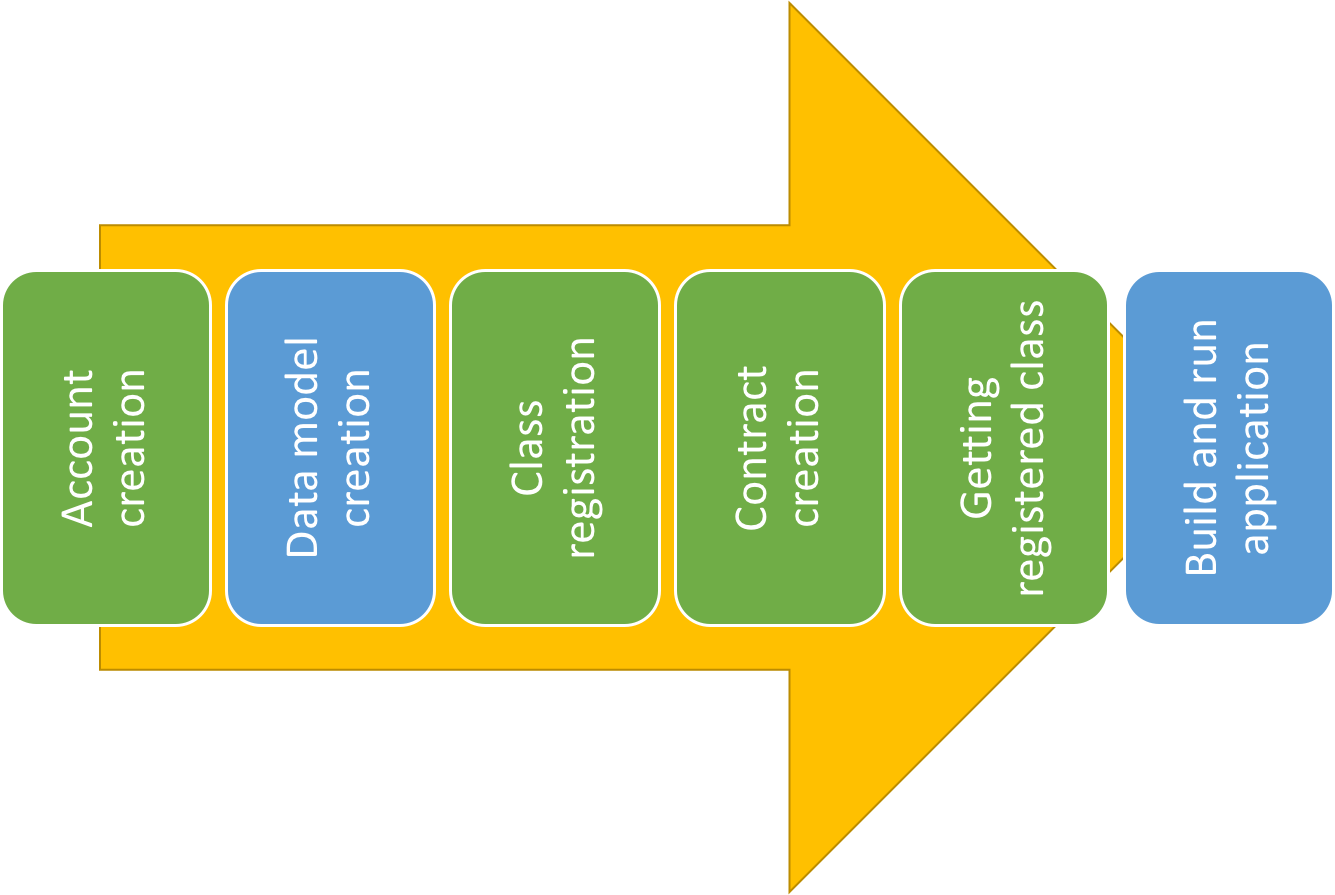
\includegraphics[scale=0.5]{FirstSteps/AppCycle.png}
\caption{Application life cycle}
\label{fig:AppCycle}
\end{figure}

\section{Account creation}\index{account}\index{account creation}

Everybody using dataClay needs to have its own account regardless of the role (model provider or application programmer). Currently accounts are identified by a string and are protected by a password. Accounts are the abstraction used to grant/deny privileges to create/use/access models and/or data.

Although dataClay foresees two different roles with respect to data, they can all be assumed by the same person and this is that case in the HelloPeople example: a single person (you) creates the model, creates application, and inserts the data.

Details on how accounts are created are presented in Chapter~\ref{sec:dClayTool}.

\section{Namespaces and class models}\index{class registration}
\label{sec:ClassRegistration}

The model provider is in charge of implementing the Java/Python class models. The involved classes are normally designed and implemented ignoring that they will be eventually used to store persistent objects in dataClay. Once the classes have been created and tested, the model provider needs to register them into dataClay to enable objects of these classes to be stored persistently.

Registering classes is important for three reasons: i) enables dataClay to automatically offer an optimal serialization of the objects instantiating any of these classes, ii) enables dataClay to execute class methods over the objects inside the backends without having to move data to the application, and iii) enables the sharing of classes among application developers in an easy and effective way.

Registering a class model only implies uploading its corresponding class files (e.g. .class files or .py files) into dataClay and defining into which namespace they should be added.

A {\bf namespace}\index{namespace} is a dataClay abstraction to group a set of classes together. Namespaces have two objectives: i) grouping related classes to ease the task of sharing them with other users and ii) avoiding class name clashing (for instance two users willing to register class models with names in common for a subset of their classes). That is, a namespace is a similar abstraction as a package in Java or module in Python.

Registering a class model can be easily performed by using the available tools described in Chapter~\ref{sec:dClayTool} and has to be performed before any application tries to store objects of this class model into dataClay.

% \section{Contract creation}\index{contract}\index{contract creation}
% 
% In order to be able to use data (actual objects) and models (classes), the application developer needs to have access to both the model and the data. In dataClay this access is allowed via model and data contracts.

% \subsection{Model contract}\index{model contract}\index{contract, model}
% 
% Model contracts allow application developers to use a given class or set of classes. These contracts can be of one of the following two types:
% 
% \begin{itemize}
% 	\item {\bf Public contract}:\index{public contract}\index{contract, public} is a contract that can be used by any dataClay user without explicit consent from the model developer. Thus any application programmer can use any class in a public contract. 
% 
% 	\item {\bf Private contract}:\index{private contract}\index{contract, private} is a contract that grants permission to use a set of classes to a specific user. Only the beneficiary user will be able to use these classes by means of this contract. A private contract may include many classes, a class may also be included in many contracts, and beneficiaries can have as many private contracts as needed to develop their applications.
% \end{itemize}
% 
% Contract creation can be easily performed by using the available tools described in Chapter~\ref{sec:dClayTool}. Once a model contract is created, dataClay will make sure that the user receiving the contract, or any user in case of a public contract, will have access to the classes included in the contract. An application can use as many models contracts as needed, and they can be a mix between public and private ones.

\section{Datasets and data contracts}\index{data contract}\index{contract, data}

In the same way we grouped classes into namespaces to ease the task of sharing them, dataClay also has the dataset abstraction. A {\bf dataset}\index{dataset} is a set of objects that will be shared with other users as a whole. Objects inside a dataset can be of any class and there is no restriction to the number of objects or their size inside a dataset. Datasets are identified by a string defined by the creator of the dataset.

Datasets can be public or private. Public datasets can be accessed by any user and they will suffice in most scenarios. On the contrary, to access a private dataset its owner has to explicitly grant permission to it. This permission granting is achieved by means of data contracts \index{data contract}. Contract creation can be easily performed by using the available tools described in Chapter~\ref{sec:dClayTool}. Once a data contract is created, dataClay will make sure that the user receiving the contract will have access to the objects included in the datasets of the contract. An application can access as many datasets as needed as will be shown in Chapter~\ref{sec:ClientConfigFiles}.

Notice that in the current public version of dataClay, only public datasets are available.

\section{Using a registered class: getting its stubs}\index{stub}\index{class stub}

As we mentioned in Section~\ref{sec:ClassRegistration}, when we implement a class model we do not take into account anything about persistence, but when using it (as seen in the code in Section~\ref{sec:HelloPeople}), persistent objects have methods such as \texttt{makePersistent}\index{makePersistent} that have not been defined as part of the class. In order to be able to use such methods, and thus enable persistence of objects, the application needs to be linked with an automatically modified version of the classes. This modified version is what we refer as {\bf stub classes}\index{stub class} or simply {\bf stubs}\index{stub}. A stub is a class file containing the modified version of the original class in order to be compatible with dataClay. It is important to understand that, besides the newly added methods, the rest of the class behaves just like the original one. 

The stubs of a class are obtained using the available tools described in Chapter~\ref{sec:dClayTool}.

\section{Build and run the application}

To run a dataClay application, we just need i) to make sure that it is using the stubs instead of the original class files and ii) to create two configuration files that specify our account, datasets, stubs path and connection info. Next section shows an example of these configuration files and Section~\ref{sec:ClientConfigFiles} describes further details.

\section{Easier than it looks}

Let's see how we can execute the examples in Sections~\ref{sec:JavaFirstApp} and~\ref{sec:PythonFirstApp}.

First, we define two configuration files. Section~\ref{sec:ClientConfigFiles} describes further details and where to place them.

The first one is named \textit{session.properties}\index{session.properties} and the initialization method (\texttt{DataClay.init()}\index{DataClay.init()} in Java or \texttt{api.init()} in Python) will automatically process it. This initialization process is detailed in Section~\ref{sec:JavaGlobalAPI} for Java and Section~\ref{sec:PythonGlobalAPI} for Python.

Here is an example:

\begin{tBox}
\begin{bash}
Account=Alice
Password=AlicePass
DataSets=HelloPeopleDS
DataSetForStore=HelloPeopleDS
StubsClasspath=./stubs
\end{bash}
\end{tBox}

A second file named \textit{client.properties}\index{client.properties} contains the basic information for the network connection with dataClay:

\begin{tBox}
\begin{bash}
HOST=127.0.0.1
PORT=11034
\end{bash}
\end{tBox}

Now you can start using a simple dataClay command line utility intended for management operations\index{management operations}. In this way, our class models can be registered, datasets with specific access rights can be defined, and our application can interact transparently with dataClay when using downloaded stubs (more details about the command line utility are explained in Chapter~\ref{sec:dClayTool}).

\begin{minipage}{\linewidth}
\begin{tBox}
\begin{bash}
 # To begin with, create an account
dataclaycmd NewAccount Alice AlicePass
 
 # Create a dataset (with granted access) 
 # to register stored objects on it
dataclaycmd NewDataContract Alice AlicePass myDataset
 
 # Register the class model in a certain namespace
 # Assuming Person.class or person.py is in ./modelClassDirPath
dataclaycmd NewModel Alice AlicePass myNamespace ./modelClassDirPath \
  <java | python>
 
 # Download the corresponding stubs for your application
dataclaycmd GetStubs Alice AlicePass myNamespace stubsDirPath
\end{bash}
\end{tBox}
\end{minipage}

